\section{Results: Survey}\label{section:Results_Survey}

\subsection{Population Selection}
We initially had two sources for our Experienced Drools users to send our survey to.
From LinkedIn we selected users who were at one degree of separation from us and listed Drools in their skills.
From StackOverflow we selected users who had asked or answered questions about Drools.

As in these two websites the users do not tend to list their contact details, some investigation was required.
From the initial selection, whose size we did not record we harvested email accounts, and failing that twitter accounts.

A few days into our survey we read a paper that described the use of academic papers as a population of expertise.
We used Google Scholar to look up Drools papers from the previous 2 years.
After skimming the papers to ensure that it was specifically about or using the Drools language we harvested emails

On the second and fourth day of the survey two subjects forwarded the weblink to the survey to mailing lists.
One, a developer from the core Drools team, sent it to a list of known Drools consultants.
The other sent it internally in his company.
both the subjects who sent the survey to their mailing list forwarded links to version C of the survey.

We had created 4 versions of the questionnaires to a combat single source bias.
We distributed the surveys to the subjects harvested from LinkedIn and StackOverflow evenly.
Because of the overrepresentation of Survey C, we distributed the subjects harvested from academic papers evenly over Surveys A, B and D.

The collection result can be seen in figure \ref{fig:Survey_participants}.
What we see here is that the method of collection did not have much of an impact on return rates.
whilst StackOverflow had a higher rate, the number of people contacted was so small that a small addition of respondents has an outsized effect on the proportion.

The first three pie charts represents the collection methods over which we had control.
These three represented 24 of our 30 completed questionnaires.
The last pie chart represents 6 completed and 4 partially completed questionnaires, that were returned from the surveys sent on by our initial participants.
We do not know the size of the starting population of these lists. 
Thus this pie chart only shows the ratio of partial to completed results.


In summary, a survey reached known 154 participants, of which 24 completed it, for a Response Rate of 15.5\%.
In addition, an unknown amount of participants were reached through mailing lists, returning a further 6 completed surveys.

\subsection{Participant demography}

Responses came from around the world.
Figure \ref{fig:Survey_locations} shows the location of the respondents were concentrated in Europe, the exceptions being the USA, Israel, and Singapore.
Italy and the Netherlands provided the largest number of responses, with 7 and 5 respectively.

\begin{figure}[H]
    \centering
    \fbox{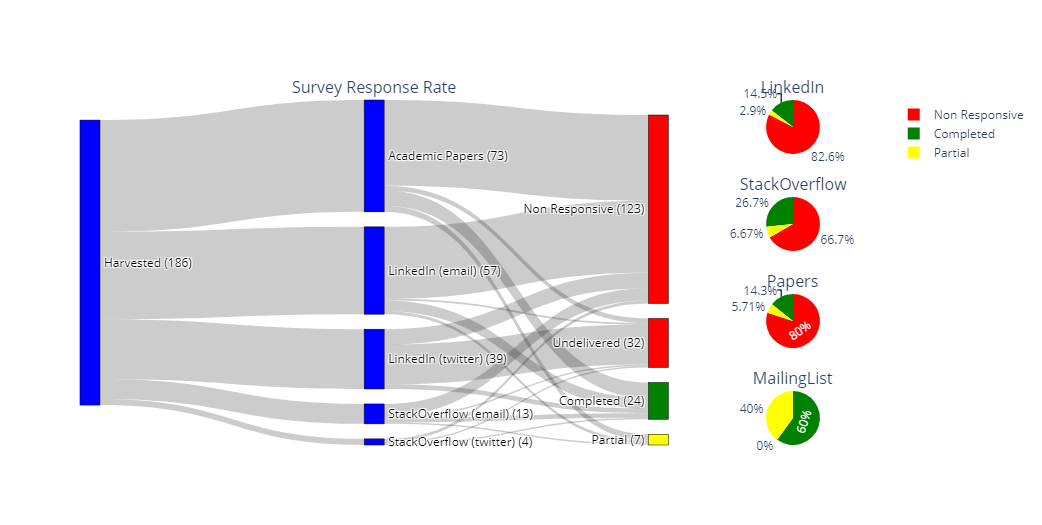
\includegraphics[width=0.95\textwidth]{Sections/images/survey_participants.png}}
    \caption{Survey Participants}
    \label{fig:Survey_participants}
\end{figure}

\begin{figure}[H]
    \centering
    \fbox{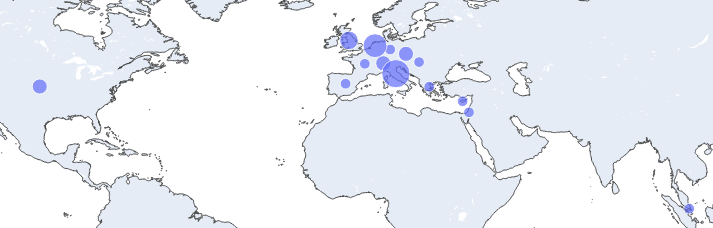
\includegraphics[width=0.95\textwidth]{Sections/images/survey_locations.png}}
    \caption{Survey Locations}
    \label{fig:Survey_locations}
\end{figure}

\begin{figure}[H]
    \begin{subfigure}{.33\textwidth}
      \centering
      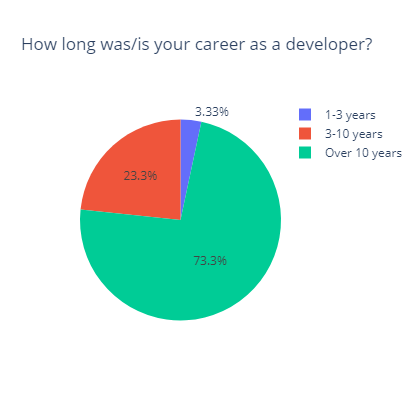
\includegraphics[width=.95\linewidth]{Sections/images/pie_experiencer.png}
      \caption{SE experience}
      \label{fig:sfig1}
    \end{subfigure}%
    \begin{subfigure}{.33\textwidth}
      \centering
      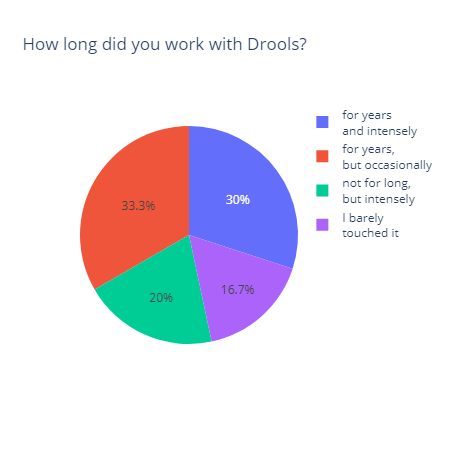
\includegraphics[width=.95\linewidth]{Sections/images/pie_droolsExperience.png}
      \caption{drools experience}
      \label{fig:sfig2}
    \end{subfigure}
    \begin{subfigure}{.33\textwidth}
        \centering
        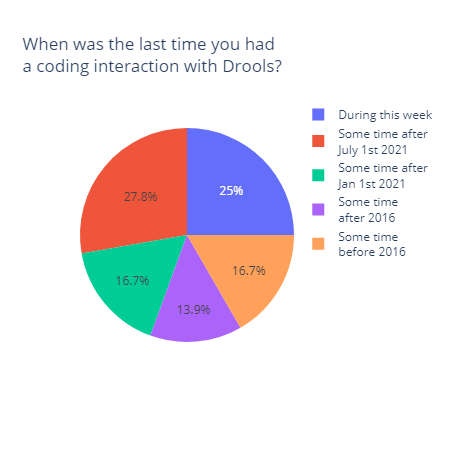
\includegraphics[width=.95\linewidth]{Sections/images/pie_recentusage.png}
        \caption{recent use}
        \label{fig:sfig3}
      \end{subfigure}
    \caption{Subject Experience}
    \label{fig:subject_experience}
\end{figure}

The experience of our subjects was quite high.
As can be seen in \ref{fig:sfig1}, most of our subjects have over 10 years programming experience.
17\% of our recipients had a low experience of Drools, and 30\% were very experienced, as shown in figure \ref{fig:sfig2}.
Figure \ref{fig:sfig3} reports that over half of our recipients have used Drools in the previous 6 weeks with only 17\% not having used Drools for more than 5 years.

Half of our subjects reported only ever using one editor for Drools, with the slight majority of those only using Eclipse.
Eclipse also had the most instances of reporting of having been used, out of the 55 instances of editors reported as being used, 20 of those were Eclipse.
There was a, to us, surprising diversity of tools being used.
The purpose of this section was to be able to calibrate responses against exposure to IDEs with greater Drools Support.
The wide diversity of editor usage and high incidence of multiple editor usage means that these answers are not suitable for use in the sub-categorisation of responses. 
The distribution of usage is shown in figure \ref{fig:editorUsage}.

\begin{figure}[h]
    \centering
    \fbox{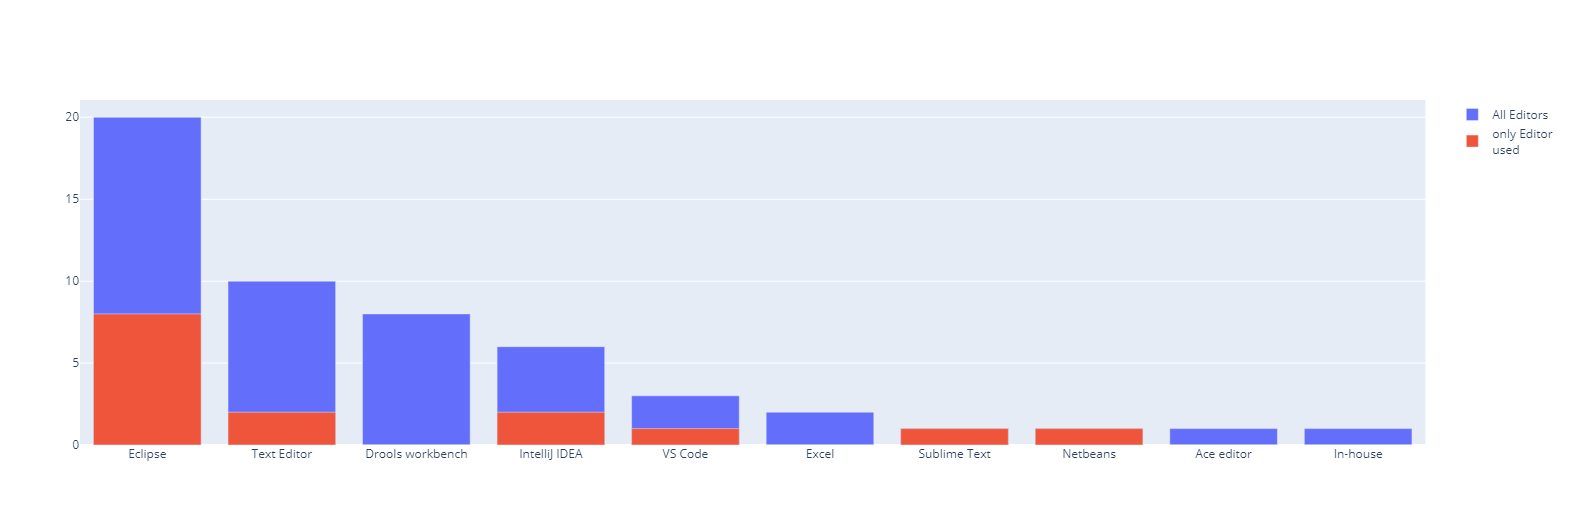
\includegraphics[width=0.95\textwidth]{Sections/images/EditorUseage.png}}
    \caption{Editors Used}
    \label{fig:editorUsage}
\end{figure}


\subsection{Question Analysis}
Until now, the choice of chart to display the survey outcome has been based on a feeling rather than research. 
The remainder of this Results sections, whilst talking about results that regard our Likert Scaled questions, we will be following the advice of Robbins et.al.\cite{robbins2011plotting} and using diverging stacked bar charts, with counts added.
This style allows the evaluation of subclasses results.
The addition of counts makes it easier to spot when the results are skewed by small numbers.

When displaying subtypes we shall split into groups.
The source of the response will create a pseudo cross-section of our participants.
The 10 who were contacted through academic papers will be considered our academics.
The remaining 20 will be considered practitioners.

The next grouping will be on Drools Experience.
The 9 who replied they had used drools ``for years and intensely'' are categorised as experts.
The 16 who either answered ``for years, but occasionally'' or ``not for long, but intensely'' are categorised as seniors.
The 5 who answered ``I barely touched it'' are categorised as novices.

Another grouping will be on recency of use.
The 12 who have used Drools in 2021 will be categorised as current users.
The remaining 18 as past users.

To remove some bias in the questionnaires we changed question order, order of projections, and which rulesets were used.
When a question is effected by this, then this will also be displayed.

\subsubsection{Question 1: First Impression}
This question shows the subject an example of projectional editing, as an animated GIF, along with an explanation.
Then she is asked her first reaction.
Figure \ref{} shows the results



